\chapter{Introduction}
\label{chap:introduction}

This chapter establishes the scope of the CORAL project. We motivate the work by characterising the state of Urdu Automatic Speech Recognition (ASR), articulate the research problem and hypothesis, present the final framing of the proposed solution as it emerged across two iterations, set the project objectives and deliverables, and document software requirements. The chapter closes with a description of how the workload was distributed across the team. The detailed methodology, implementation, and empirical evaluation are deferred to Chapters~\ref{chap:approach} and~\ref{chap:implementation}.

\section{Background}
\label{sec:background}

Automatic Speech Recognition has experienced extraordinary progress over the past decade. Foundation models such as OpenAI's Whisper~\cite{radford2022whisper}, Meta's MMS~\cite{pratap2023mms}, and Meta's SeamlessM4T~\cite{seamlessm4t2023} now achieve sub-5\% Word Error Rate (WER) on widely-spoken languages such as English and Mandarin. This performance has unlocked production deployments in voice assistants, real-time captioning, healthcare dictation, and dictation-based accessibility tools.

Urdu is the national language of Pakistan, an official language of several Indian states, and the lingua franca of the South Asian subcontinent. It is spoken by more than 230~million people worldwide and is written in the Nastaliq variant of the Perso-Arabic script. Despite its demographic significance, Urdu remains severely under-represented in modern ASR research. The most comprehensive recent benchmark of multilingual ASR systems on Urdu, conducted by Arif et al.~\cite{arif2024wer}, reports that even the strongest models achieve WER above 13\% on read speech and approaching 20\% on conversational audio. This performance ceiling places critical Urdu ASR applications in healthcare, legal documentation, education, and assistive technology effectively out of reach.

Urdu poses several genuine difficulties to ASR systems that are absent from high-resource languages:

\begin{itemize}
  \item \textbf{Limited training data.} High-quality, large-scale, time-aligned Urdu speech corpora are scarce compared with English or Mandarin. Most multilingual models see Urdu only as a small minority of their training mixture.
  \item \textbf{Linguistic complexity.} Urdu has rich morphology, extensive use of loanwords from Arabic, Persian, and English, an elaborate verbal agreement system covering gender, number and case, and pervasive optional diacritics that are produced inconsistently by different ASR back-ends.
  \item \textbf{Code-switching.} Conversational Pakistani speech routinely alternates between Urdu and English at the word and phrase level, a distribution that monolingual ASR systems are not trained to handle.
  \item \textbf{Dialectal variation.} Multiple regional dialects with distinct acoustic and lexical properties coexist within both Pakistan and India.
  \item \textbf{Script heterogeneity.} The same phoneme can be represented by multiple Unicode code points drawn from both the Arabic and Urdu sub-blocks (e.g.\ Arabic KAF \texttt{U+0643} vs.\ Urdu KEHEH \texttt{U+06A9}). This causes word-level mismatches during alignment and WER computation even when the word is phonetically and semantically correct.
  \item \textbf{Word-boundary inconsistency.} Urdu ASR back-ends disagree systematically on word boundaries: a phrase that one model transcribes as a single token is often split into two or three tokens by another, or merged from multiple tokens into one. Naive word-level alignment misinterprets these segmentation events as substitutions or deletions, corrupting any downstream voting or fusion signal.
\end{itemize}

\subsection{Limitations of Single-Model and Naive-Ensemble ASR}
\label{ssec:single-model-limits}

Single-model ASR architectures, even when fine-tuned on Urdu, suffer from three well-documented limitations: (i)~\emph{deterministic predictions} -- they emit a single best hypothesis without considering plausible alternatives; (ii)~\emph{absent uncertainty signal} -- they provide no easily actionable mechanism to indicate confidence in their output; and (iii)~\emph{domain brittleness} -- models fine-tuned on read speech generalise poorly to conversational audio, code-switched speech, or dialectal variation. The natural response is to combine the outputs of several independently trained ASR systems, expecting that the errors of one model will be corrected by the consensus of others. This is appealing because it requires no retraining, can be deployed at inference time, and can leverage architecturally diverse models that make systematically different error types.

However, ensemble combination methods such as ROVER~\cite{fiscus1997rover} were designed for phonetically regular, space-delimited scripts such as English. Applied naively to Urdu, they fail in three concrete ways: they are confounded by Arabic--Urdu Unicode variants; they misinterpret word-boundary disagreements as deletions or insertions; and they degrade quality when the ensemble contains models of widely heterogeneous quality (the canonical ROVER failure mode). The CORAL project was motivated by the observation that solving these three Urdu-specific complications requires a purpose-built post-processing pipeline rather than a direct application of off-the-shelf ensemble methods.

\section{Problem Statement}
\label{sec:problem}

CORAL addresses the following research problem:

\begin{quote}
\itshape
Current state-of-the-art pre-trained ASR models for Urdu exhibit Word Error Rates between 13\% and 20\% on read and conversational benchmarks respectively, and degrade further on out-of-domain and code-switched speech. No widely available ASR back-end provides robust handling of Arabic--Urdu Unicode variation, word-boundary disagreement across architectures, or out-of-vocabulary proper nouns. Existing ensemble fusion techniques developed for English are not directly transferable, because they confound Unicode variants, segmentation disagreement, and quality heterogeneity. The community needs a post-processing pipeline that recovers from these failures at inference time, without requiring fine-tuning or any change to the underlying acoustic models.
\end{quote}

This research problem decomposes into three concrete challenges:

\begin{enumerate}
  \item \textbf{Script heterogeneity and segmentation disagreement.} Word-boundary inconsistency is not captured by word-level alignment alone, and Arabic--Urdu Unicode variation causes phonetically identical tokens to register as distinct words during voting and WER computation.
  \item \textbf{Out-of-vocabulary handling.} Proper nouns, named entities, and rare technical terms are systematically misrecognised by all available ASR back-ends but are precisely the tokens whose correct transcription matters most in downstream applications.
  \item \textbf{Linguistic coherence and code-switching.} Word-level voting, even when correctly aligned, cannot recover sentence-level fluency, restore code-switched English tokens, or resolve grammatical agreement errors that span longer than a few words.
\end{enumerate}

\subsection{Research Hypothesis}
\label{ssec:hypothesis}

\textit{The CORAL hypothesis}: Combining (i)~Urdu-specific Unicode normalisation, (ii)~weighted split-merge-aware alignment of multiple ASR hypotheses, (iii)~hybrid OOV detection and correction with BK-tree fuzzy lookup ranked by an n-gram language model, (iv)~conservative position-wise voting, and (v)~targeted LLM refinement of the voted output, is sufficient to substantially reduce WER over the strongest single-model baseline on both read-speech and conversational Urdu, without requiring any fine-tuning of the underlying acoustic models.

\section{Proposed Solution: Evolution of the CORAL Framework}
\label{sec:proposed-solution-overview}

The CORAL system was developed across two distinct iterations of the Final Year Project, and the framework's framing evolved meaningfully between them. We document this evolution explicitly so that the relationship between the FYP-1 design and the deployed FYP-2 system is unambiguous; the technical detail behind the final pipeline is presented in Chapter~\ref{chap:approach}.

\subsection{Iteration~1 Framing (FYP-1): ``Generate-and-Refine''}
\label{ssec:iter1-framing}

The original CORAL framing, presented in the FYP-1 final report, was a two-stage \emph{Generate-and-Refine} architecture. \textbf{Stage~1} deployed an ensemble of pre-trained ASR models (Whisper Large/Medium/Small and Wav2Vec2-XLSR Urdu), extracted architecture-specific word-level confidence scores from each, and produced four to five confidence-annotated hypotheses for each audio input. \textbf{Stage~2} fed these confidence-annotated hypotheses into a black-box instruction-tuned LLM (Alif-1.0-8B-Instruct, an Urdu-focused 8B-parameter model) using a structured prompt that asked the LLM to weight competing tokens by their reported confidences and emit a single corrected sentence. Iteration~1 established a strong baseline (Whisper-Large at 17.76\% WER on a 10-clip read-speech test set) and validated that the architecture-specific confidence-extraction methodology produced usable signals; Iteration~2 then implemented the LLM-correction stage and reported a 18.15\% WER on a controlled 20-sample synthetic dataset that probed three calibration regimes (well-calibrated, overconfident, underconfident) and three error types (substitution, insertion, deletion).

\subsection{Iteration~2 Reframing (FYP-2): A Five-Stage Post-Processing Pipeline}
\label{ssec:iter2-reframing}

Several findings from Iteration~1 motivated a deliberate redesign for Iteration~2. The synthetic 20-sample evaluation revealed that the LLM stage performed adequately on substitution errors but poorly on deletion errors and was sensitive to confidence calibration; raw confidence scores from heterogeneous architectures lived on incompatible scales; and the controlled experiment did not expose the system to two failure modes that proved dominant on real ASR output --- Arabic--Urdu Unicode conflation and word-boundary disagreement across models. Iteration~2 therefore reframed CORAL from a two-stage Generate-and-Refine system into a five-stage post-processing pipeline (Stages~0--4) and made the following deliberate choices:

\begin{itemize}
  \item \textbf{A dedicated normalisation stage (Stage~0)} was introduced to handle Arabic--Urdu Unicode conflation, diacritic removal, tatweel removal, and punctuation stripping. Normalisation alone delivers a 1.9-WER-point reduction on conversational Urdu --- a zero-cost, zero-risk gain that was invisible to the FYP-1 evaluation setup.
  \item \textbf{A weighted split-merge-aware alignment algorithm (Stage~1)} replaced the implicit alignment performed by the LLM. The weighted alignment makes word-boundary disagreement explicit and exposes SAME/SPLIT/MERGE/NOISE metadata that downstream stages can act on.
  \item \textbf{An OOV detection and correction stage (Stage~2)} based on a BK-tree~\cite{burkhard1973bk} over a half-million-word Urdu vocabulary corpus, ranked using bi/tri-gram context, was introduced to recover named entities and rare words.
  \item \textbf{Position-wise majority voting with conservative tie-breaking (Stage~3)} replaced the LLM as the primary mechanism for resolving disagreement on common, in-vocabulary words.
  \item \textbf{The LLM stage (Stage~4)} was retained but repositioned: rather than acting as the primary fusion mechanism over confidence-annotated hypotheses, it now acts as a final refinement layer over the already-voted transcript, addressing fluency, code-switching, and named-entity contexts that lexical voting cannot recover. The LLM was also changed from Alif-1.0-8B-Instruct to commercial frontier models (Anthropic's Claude Sonnet, Google's Gemini, OpenAI's GPT-4o through OpenRouter) accessed via the front-end, which deliver more reliable instruction following.
\end{itemize}

\subsection{Components Dropped from the FYP-1 Design}
\label{ssec:dropped-components}

For full clarity, the following FYP-1 design elements were intentionally dropped, replaced, or de-emphasised in the final FYP-2 system:

\begin{itemize}
  \item \textbf{Word-level confidence extraction from Whisper and Wav2Vec2.} Architecture-specific confidence-score extraction was a centrepiece of the FYP-1 design. The deployed FYP-2 pipeline does not use these scores in its server-side voting or alignment logic; calibrated cross-architecture confidence proved unreliable in practice and is replaced with a static, model-quality--based confidence weighting applied only by the front-end LLM stage.
  \item \textbf{Expected Calibration Error (ECE) as a primary metric.} ECE was used in FYP-1 to compare the confidence quality of individual ASR back-ends. It is not used in the FYP-2 evaluation, which reports WER and CER only on the deployed pipeline. The findings from FYP-1's ECE analysis are reported in Section~\ref{sec:iter1-results} as historical context.
  \item \textbf{Synthetic 20-sample evaluation with calibration regimes.} The synthetic substitution/insertion/deletion injection used in FYP-1 was a useful Stage-2 isolation test but proved to be a poor proxy for real ASR error distributions. FYP-2 evaluates on real ASR output over 2{,}995 Common Voice utterances (read speech) and 500 Conversational Urdu clips.
  \item \textbf{Alif-1.0-8B-Instruct as the Stage-2 LLM.} Replaced with commercial frontier models that are accessed client-side, reducing GPU requirements on the backend and improving instruction-following quality.
  \item \textbf{The two-stage ``Generate-and-Refine'' framing.} Reframed as a five-stage pipeline (Stages~0--4) in which the LLM is the \emph{last} stage rather than the only consumer of multi-model hypotheses.
\end{itemize}

\subsection{Final Architecture at a Glance}
\label{ssec:final-arch-glance}

The final CORAL system is delivered as a \texttt{FastAPI} backend exposing three pipeline endpoints (\texttt{/align}, \texttt{/oov}, \texttt{/correct}) plus a model registry, a \texttt{Next.js} React front-end implementing a four-pass user workflow (mode selection, alignment, OOV sieve scan, correction), and Kaggle GPU notebooks that self-register through ngrok-tunnelled HTTPS endpoints to provide live ASR inference. The full architecture is described in Chapter~\ref{chap:approach} and Chapter~\ref{chap:implementation}.

\begin{figure}[h]
    \centering
    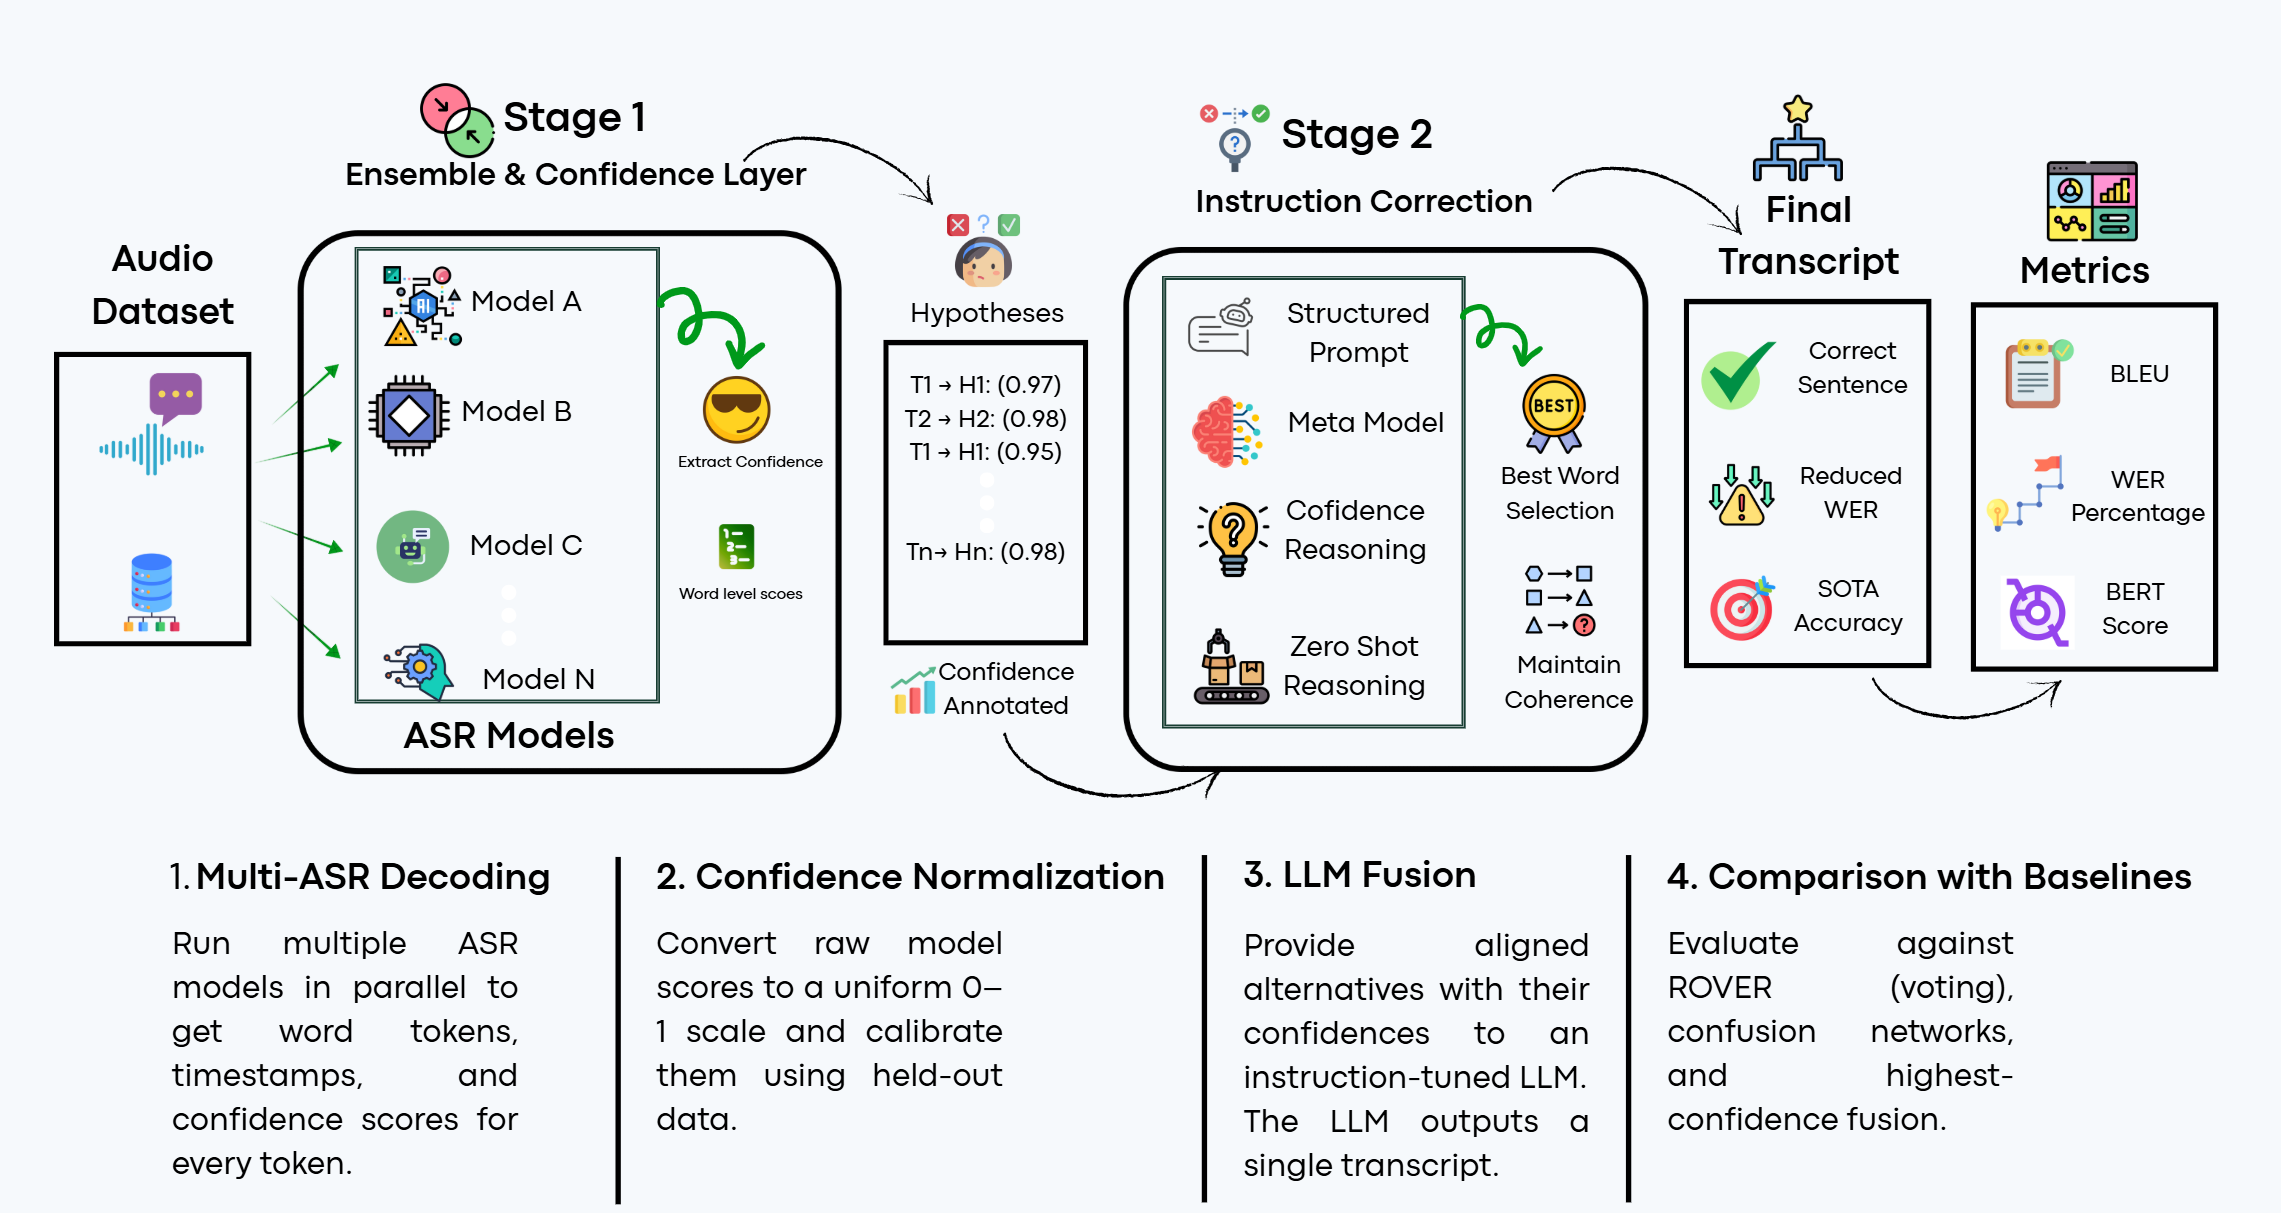
\includegraphics[width=0.95\textwidth]{ThesisFigs/coral_architecture.png}
    \caption{CORAL conceptual architecture as introduced in FYP-1: a two-stage Generate-and-Refine pipeline. The deployed FYP-2 system reorganises this concept into five sequential stages with the LLM repositioned as a refinement layer; the deployed pipeline is shown in Figure~\ref{fig:coral-pipeline}.}
    \label{fig:coral-architecture-iter1}
\end{figure}

\section{Project Objectives and Scope}
\label{sec:objectives}

The objectives of the CORAL project, as finalised after the FYP-1 evaluation, are:

\begin{enumerate}
  \item Design and implement a robust Urdu normalisation module covering diacritic removal, the seven canonical Arabic--Urdu character mappings, tatweel removal, punctuation stripping, ASCII removal, and whitespace normalisation.
  \item Design and implement a split-merge-aware alignment algorithm that aligns word sequences using weighted Levenshtein distance and classifies each aligned chunk as SAME, SPLIT, MERGE, or NOISE.
  \item Develop an OOV detection and correction module combining BK-tree fuzzy lookup with bi/tri-gram language-model candidate ranking over a $\sim$500K-word Urdu vocabulary corpus.
  \item Implement a position-wise majority voting corrector with explicit handling of insertion offsets and conservative tie-breaking.
  \item Integrate an LLM refinement layer for fluency restoration, code-switching recovery, and named-entity handling, accessed via the front-end through commercial LLM APIs.
  \item Deploy the pipeline as a REST API (FastAPI) with three endpoints, fronted by a Next.js + React user interface implementing a four-pass workflow with both file-upload and live-speech modes.
  \item Conduct a thorough empirical evaluation and ablation study on publicly available Urdu ASR benchmarks, isolating the contribution of each component.
\end{enumerate}

\subsection{Deliverables}
\label{ssec:deliverables}

The project delivers the following artefacts:

\begin{itemize}
  \item A complete five-stage CORAL post-processing pipeline implemented in Python, deployed as a \texttt{FastAPI} service with Docker support.
  \item A Next.js + React front-end implementing the four-pass user workflow, with both file-upload and live-recording entry modes, animated alignment-scan and OOV-sieve visualisations, and side-by-side correction diff views.
  \item Kaggle GPU notebooks that self-register through an ngrok HTTPS tunnel and provide live transcription endpoints for Whisper-Large-v3 and SeamlessM4T-v2-Large.
  \item A model registry with 60-second heartbeats and 300-second silent eviction, accessible via authenticated registry tokens.
  \item A reproducible evaluation framework producing both WER and CER metrics across all four pipeline configurations (\texttt{untouched}, \texttt{norm\_baseline}, \texttt{robust}, \texttt{rrf}) for every ensemble member, exported as a tab-separated value file (\texttt{asr\_evaluation/ensemble\_correction\_eval.tsv}).
  \item A reference Urdu vocabulary, BK-tree, and bi/tri-gram corpus shipped via HuggingFace Hub and loaded into DuckDB at server startup.
  \item Comprehensive documentation including this report, the FYP-1 and FYP-2 reports, architecture diagrams, and source-level documentation in the codebase.
\end{itemize}

\section{Software Requirements Specification}
\label{sec:srs}

CORAL is realised as a software system, and its requirements are recorded here for completeness. The functional requirements are organised by module, and the non-functional requirements describe end-to-end qualities of the deployed system.

\subsection{Functional Requirements}
\label{ssec:func-req}

\textbf{FR1 -- Normalisation Service.}
\begin{itemize}[nosep]
  \item FR1.1: The system shall accept arbitrary UTF-8 Urdu text input.
  \item FR1.2: The system shall strip Unicode diacritics in the ranges \texttt{U+0610}--\texttt{U+061A} and \texttt{U+064B}--\texttt{U+065F}, plus the superscript alef (\texttt{U+0670}).
  \item FR1.3: The system shall apply the seven canonical Arabic-to-Urdu character substitutions defined in Appendix~\ref{app:unicode-table}.
  \item FR1.4: The system shall remove the tatweel (\texttt{U+0640}), zero-width and directional control characters, Arabic and Urdu punctuation, ASCII punctuation and digits, and ASCII letters; consecutive whitespace shall be collapsed.
\end{itemize}

\textbf{FR2 -- Multi-Model Alignment Service (\texttt{POST /align}).}
\begin{itemize}[nosep]
  \item FR2.1: The system shall accept an arbitrary number of named ASR hypotheses with one designated source model.
  \item FR2.2: The system shall produce per-position word-level alignment labels (MATCH, SUBSTITUTION, DELETION, INSERTION) using weighted Levenshtein distance.
  \item FR2.3: The system shall produce per-position split-merge metadata (SAME, SPLIT, MERGE, NOISE) using a character-level secondary alignment.
  \item FR2.4: The system shall return both source-side and target-side metadata views in the response.
\end{itemize}

\textbf{FR3 -- OOV Detection and Candidate Ranking Service (\texttt{POST /oov}).}
\begin{itemize}[nosep]
  \item FR3.1: The system shall flag a word as OOV iff it appears in exactly one model's normalised output \emph{and} its corpus frequency is below a configurable threshold (default 2{,}000).
  \item FR3.2: For each flagged token, the system shall retrieve candidates from a BK-tree using a length-adaptive edit-distance threshold.
  \item FR3.3: The system shall rank candidates lexicographically by edit-distance, unigram presence, trigram-context hits, bigram-context hits, and corpus frequency.
  \item FR3.4: The top-$K$ candidates per token (default $K=10$) shall be returned with all ranking signals.
\end{itemize}

\textbf{FR4 -- Voting Correction Service (\texttt{POST /correct}).}
\begin{itemize}[nosep]
  \item FR4.1: For each source position not flagged as OOV, the system shall collect votes from all companion models, skipping insertion-aligned slots.
  \item FR4.2: The plurality winner shall replace the source word only if it is unique; on ties, the source word shall be preserved (conservative tie-break).
  \item FR4.3: For each flagged OOV position, the source word shall be replaced by the top-ranked OOV candidate.
  \item FR4.4: The response shall include the corrected sentence, the source sentence, and a position-indexed diff.
\end{itemize}

\textbf{FR5 -- Model Registry.}
\begin{itemize}[nosep]
  \item FR5.1: A Kaggle GPU notebook shall be able to register itself with name, HTTPS endpoint, and session ID via \texttt{POST /registry/register}, authenticated with a registry token.
  \item FR5.2: A registered model shall send heartbeats every 60~seconds via \texttt{POST /registry/ping}; the registry shall evict models silent for more than 300~seconds.
  \item FR5.3: \texttt{POST /registry/transcribe} shall accept an audio file, source-model name, and whitelist of companion models, fan out the request to live registered models in parallel with a 60-second timeout, and return all collected transcripts.
  \item FR5.4: \texttt{GET /registry/models} shall list currently-live models with their session IDs and seconds-since-last-ping.
\end{itemize}

\textbf{FR6 -- Front-End Workflow.}
\begin{itemize}[nosep]
  \item FR6.1: The user shall be able to choose between \emph{File} mode (CSV/TSV/JSON upload) and \emph{Speech} mode (file upload or in-browser recording).
  \item FR6.2: The front-end shall display a four-phase animated OOV-sieve scan over the alignment output (sieve cursor, word colouring, character-level expansion, structural metadata colouring).
  \item FR6.3: OOV words shall be displayed with a rose dotted underline; clicking shall reveal the ranked candidate list with all ranking columns.
  \item FR6.4: The correction stage shall offer two modes: \emph{Voting} (server-side \texttt{POST /correct}) and \emph{LLM} (client-side Gemini or OpenRouter) with provider selection and dynamic model-list fetch.
\end{itemize}

\subsection{Non-Functional Requirements}
\label{ssec:nonfunc-req}

\textbf{Performance.}
\begin{itemize}[nosep]
  \item PER-1: The \texttt{/align} endpoint shall complete in under 1~second on a typical Urdu utterance of 5--20 words, on commodity CPU hardware.
  \item PER-2: The BK-tree shall be loaded from a serialised joblib file in under 10~seconds on first startup.
  \item PER-3: BK-tree fuzzy search shall be at least an order of magnitude faster than a linear scan over the vocabulary.
  \item PER-4: \texttt{/registry/transcribe} fan-out shall enforce a 60-second per-model timeout and complete with the partial results of any models that responded.
\end{itemize}

\textbf{Reliability.}
\begin{itemize}[nosep]
  \item REL-1: A failure of any one ASR back-end during fan-out shall not prevent CORAL from delivering a corrected transcript using the surviving back-ends.
  \item REL-2: Models silent for more than 300 seconds shall be automatically evicted from the registry.
\end{itemize}

\textbf{Security.}
\begin{itemize}[nosep]
  \item SEC-1: Registration and heartbeat endpoints shall require a shared \texttt{X-Registry-Token}.
  \item SEC-2: The transcribe endpoint shall require a shared \texttt{X-API-Token}.
  \item SEC-3: Registered endpoint hostnames shall be validated against an explicit allowlist (default \texttt{ngrok-free.app}, \texttt{ngrok.io}).
  \item SEC-4: Audio uploads shall be size-bounded (default 25~MB).
\end{itemize}

\textbf{Usability.}
\begin{itemize}[nosep]
  \item USE-1: The user shall be able to complete the full alignment $\to$ OOV $\to$ correction workflow without manually invoking any backend endpoint.
  \item USE-2: The OOV sieve animation shall complete in less than 4~seconds for a 30-word utterance.
  \item USE-3: All operations shall be persisted to \texttt{localStorage} so that page refreshes preserve user state.
\end{itemize}

\section{Report Organisation}
\label{sec:report-org}

The remainder of this report is organised as follows:

\begin{itemize}
  \item \textbf{Chapter~\ref{chap:litreview}} presents a literature review covering Urdu ASR benchmarking, ASR ensemble methods (ROVER and successors), confidence estimation, LLM-based ASR post-correction, multi-task and multi-modal ASR, BK-trees for fuzzy string search, and a head-to-head comparison with the closest concurrent system, Multi-ASR + SpeechLLM. We also tabulate research gaps and explain how CORAL addresses each.
  \item \textbf{Chapter~\ref{chap:approach}} details the proposed approach: the five-stage pipeline architecture, the normalisation module, the weighted split-merge-aware alignment algorithm, the OOV detection and ranking module, the consensus voting algorithm, and the LLM refinement layer. Each stage is presented with a pseudo-code algorithm and a worked example.
  \item \textbf{Chapter~\ref{chap:implementation}} covers implementation, evaluation methodology, results, and the full ablation study. We describe the technology stack, REST API design, BK-tree construction, the four-pass front-end workflow, the Iteration~1 baseline experiments, and the Iteration~2 evaluation on Common Voice (read speech) and Conversational Urdu. We then present the seven-step ablation (C0--C7) attributing the WER reduction to specific components.
  \item \textbf{Chapter~\ref{chap:conclusion}} concludes the report and outlines future work.
  \item \textbf{Appendix~\ref{app:unicode-table}} contains the Unicode normalisation table, while \textbf{Appendix~\ref{app:api-spec}} contains the REST API specifications.
\end{itemize}

\section{Work Distribution}
\label{sec:work-dist}

The CORAL project was developed by a three-member team. The work distribution evolved across the two iterations and matches the deliverables described above.

\begin{table}[h]
    \centering
    \renewcommand{\arraystretch}{1.3}
    \begin{tabularx}{\textwidth}{p{4cm}p{2cm}X}
    \toprule
    \textbf{Member} & \textbf{Roll No.} & \textbf{Primary Responsibilities} \\
    \midrule
    Ali Irfan & 21I-2572 & Lead developer of the post-processing pipeline. Designed and implemented the Stage~1 weighted split-merge-aware alignment algorithm, the BK-tree data structure, the OOV detection criterion, the candidate ranking and voting logic in \texttt{coral\_pipeline\_functions.py}, and the FastAPI \texttt{/align}, \texttt{/oov}, and \texttt{/correct} endpoints. Authored the n-gram corpus generation pipeline (\texttt{generate\_ngrams.ipynb}) and DuckDB integration. \\
    Nouman Hafeez & 21I-0416 & Evaluation lead and LLM integration. Built the Iteration~1 multi-model evaluation framework (WER, CER, confidence, ECE) and the Iteration~2 evaluation pipeline (\texttt{ensemble\_correction\_eval.tsv}). Implemented memory management and Kaggle deployment notebooks (\texttt{whisper\_large\_kaggle.ipynb}, \texttt{seamless\_large\_kaggle.ipynb}), the model registry with eviction sweep, and authored the LLM prompts and provider integration logic (Gemini, OpenRouter). Coordinated the dataset assembly (Common Voice extraction, Conversational Urdu sampling) and per-stage WER measurement. \\
    Rafay Khattak & 21I-0423 & Front-end and user-experience lead. Implemented the Next.js + React front-end (\texttt{ModeSelector}, \texttt{Pass0Speech}, \texttt{Pass1Input}, \texttt{Pass2Sieve}, \texttt{Pass3Correction}), the typed API client (\texttt{lib/api.ts}), the four-phase OOV sieve animation, and the side-by-side voting/LLM correction views. Authored the Iteration~1 Flask web interface and contributed to the design of the Stage~4 LLM correction prompt format. \\
    \bottomrule
    \end{tabularx}
    \caption{Work distribution across the three-member team.}
    \label{tab:work-distribution}
\end{table}

All members participated in the literature survey, the ablation study experimental design, dataset annotation and verification, and the writing of this report. Code review was performed via pair-programming sessions and pull-request comments throughout development.

\section{Summary}
\label{sec:ch1-summary}

This chapter has motivated CORAL by establishing the persistent performance gap between Urdu ASR and high-resource-language ASR, articulated three concrete challenges (script heterogeneity, OOV handling, and linguistic coherence) that single-model and naive-ensemble approaches do not solve, traced the evolution of the framework from a two-stage Generate-and-Refine design (FYP-1) to a five-stage post-processing pipeline (FYP-2), made explicit the components that were intentionally dropped in the redesign, set the project objectives and deliverables, recorded the software requirements, and presented the work distribution. The next chapter situates CORAL in the broader literature.
